\documentclass[12pt,a4paper,ngerman,openany]{report}
\usepackage{babel}       
%\usepackage{natbib}
\usepackage{url}
%\usepackage[ansinew]{inputenc}
\usepackage{amsmath}
\usepackage{nicefrac} % macht schöne Brüche mit querstrich mit \nicefrac{1}{2}
\usepackage{graphicx}
%\graphicspath{}
% \usepackage{parskip}  % raus damit
\setlength{\parindent}{15pt}
\setlength{\parskip}{0pt}
\usepackage{fancyhdr}
\setlength{\headheight}{15pt}
\usepackage{amsfonts}
\usepackage{float}
\usepackage{caption}
\usepackage{subcaption} 
\usepackage[T1]{fontenc} %sorgt für richtige Zeilenumbrüche
\usepackage{pdfpages} % mehrseitige pdf einbinden
\usepackage{listings} 
\lstset{ breaklines=true}
\usepackage{csquotes}

\usepackage[backend=biber,style=authoryear]{biblatex}
\addbibresource{literatur.bib}


\usepackage{pgfplots} %für plots
\pgfplotsset{compat=newest}

\usepackage{pdfpages} % lässt andere PDFs einbinden mit \includepdf[pages=-]{myfile.pdf}
\usepackage{varioref} % macht mit \vref{} viel bessere referenzen
%\usepackage{hyperref} % macht klickbare referenzen
\usepackage[hidelinks]{hyperref}

\usepackage{xcolor, soul} %mit \hl{} kann man toll Sachen hervorheben.
\newcommand{\highlight}[1]{%
  \colorbox{yellow!50}{$\displaystyle#1$}} % mit \highlight{} kann man sogar in Gleichungen hervorheben 

\usepackage{vmargin}
\usepackage[section]{placeins}
\usepackage{capt-of}
\usepackage{enumitem}
\usepackage{multirow}
\usepackage{blindtext}
\usepackage[version=4]{mhchem} % um Chemische Elementsymbole zu benutzen

%spread to latex:
\usepackage{booktabs, multirow} % for borders and merged ranges
\usepackage{changepage,threeparttable} % for wide tables
\setlength{\parindent}{15pt} %absätze einrücken

\providecommand{\e}[1]{\ensuremath{\cdot 10^{#1}}}
\providecommand{\fehlt}{\textcolor{red}{\emph{Fehlt!\dots}}}

\usepackage{siunitx}
\sisetup{
	locale = DE ,
	separate-uncertainty = true,
	%per-mode = fraction,
	%per-mode = symbol
}
\DeclareSIUnit\bar{bar}



\setmarginsrb{3 cm}{2.5 cm}{3 cm}{2.5 cm}{1 cm}{1.5 cm}{1 cm}{1.5 cm}
\title{Neuronales Netz für den\\[0.5cm] kalifornischen Hauspreis-Datensatz}	
\newcommand{\shorttitle}{Neuronales Netz für den kalifornischen Hauspreis-Datensatz}
% Title

\author{Felix Hollfoth}				
% Author
\date{\today}
% Date

\makeatletter
\let\thetitle\@title
\let\theauthor\@author
\let\thedate\@date
\makeatother

\pagestyle{fancy}
\fancyhf{}

\rhead{\theauthor}
\lhead{\shorttitle}
\cfoot{\thepage}
%%%%%%%%%%%%%%%%%%%%%%%%%%%%%%%%%%%%%%%%%%%%
\begin{document}
	
%%%%%%%%%%%%%%%%%%%%%%%%%%%%%%%%%%%%%%%%%%%%%%%%%%%%%%%%%%%%%%%%%%%%%%%%%%%%%%%%%%%%%%%%%

\begin{titlepage}
    \centering
    \vspace*{0.5 cm}
    % \begin{large} Justus-Liebig-Universität\\ Gießen \end{large}
    
\includegraphics[width = 0.6 \textwidth]{Bilder/JLU_Giessen-Logo}	%University Logo
    \\[2.0 cm]
    % \begin{center}    \textsc{\Large Justus - Liebig - Universität}\\{Giessen}\\[0.8cm]	\end{center}% University Name
    
    \textsc{\Large Gruppennummer: 308}  \\[0.3 cm]				% Course Code
    \rule{\linewidth}{0.2 mm} \\[0.2 cm]
    { \huge \bfseries \thetitle}\\
    \rule{\linewidth}{0.2 mm}\\[2.0 cm]
    
    
    \begin{minipage}{0.5\textwidth}
        \begin{flushleft}
            \emph{Übrige Gruppenmitglieder:}\\
            \large{Florian Adamczyk}\\
            \large{Björn Becker}\\
            \large{Felix Neumann (Sprecherin)}\\
            \large{Kolja Scriba}\\
            %  Affiliation\\
        \end{flushleft}
    \end{minipage}~
    \begin{minipage}{0.5\textwidth}
        \begin{flushright}
            
            \emph{Protokoll von:} \\
            
            \large{Felix Hollfoth}\\ 
            \small{\href{mailto:felix.hollfoth@stud.uni-giessen.de}{felix.hollfoth@stud.uni-giessen.de}\\
                Matrikel Nr.: 8221324\: }\\[0.5cm]
            
        \end{flushright}
    \end{minipage}\\[2.0 cm]

        
    \begin{minipage}{0.8\textwidth}
       \begin{center}
        \large
        Modul: Künstliche Intelligenz I\\
        Dozent: Prof. Dr. Christian Heiliger\\
        Semester: Wintersemester 2025/26
        \end{center} 
    \end{minipage}

\vfill

\end{titlepage}

%%%%%%%%%%%%%%%%%%%%%%%%%%%%%%%%%%%%%%%%%%%%%%%%%%%%%%%%%%%%%%%%%%%%%%%%%%%%%%%%%%%%%%%%%
\setcounter{secnumdepth}{3} 
\setcounter{tocdepth}{4}
%\clearpage
%\thispagestyle{plain}
%\tableofcontents
\cleardoublepage
\tableofcontents
\cleardoublepage


%\newpage

%%%%%%%%%%%%%%%%%%%%%%%%%%%%%%%%%%%%%%%%%%%%%%%%%%%%%%%%%%%%%%%%%%%%%%%%%%%%%%%%%%%%%%%%%
\renewcommand{\thesection}{\arabic{section}}

\newpage

\section{Logbuch}




\newpage
\section{Zusammenfassung des Logbuchs}
\subsection{Ausgangssituation}
Mit dem Ziel ein neuronales Netz basierenden auf dem California Housing Datensatz von Scikit Learn zu entwickeln, wird Tensorflow bzw. Keras zum Modelltraining verwendet.

Hilfsfunktionen sind bereits programmiert, wodurch der Datensatz eingelesen und bereinigt wird. Ebenfalls liegen Funktionen zum generieren einheitlicher Datensplits und für einheitliche Metriken zum Ergebnisvergleich vor. Ein erstes Modell zur Einschätzung des neuronalen Netzes gegenüber der linearen Regression liegt bereits vor. \parencite{florians_code}

Meine zentrale Aufgabe lautet nun dieses Netz bezüglich ausgewählter Hyperparameter zu Verbessern und deren Einfluss auf das Lernen des Netzes zu untersuchen.

\subsection{Variation von Hyperparametern am neuronalen Netz}
Aus vorherigen Analysen \parencite{florians_code} geht hervor, dass den Daten ein nichtlinearer Zusammenhang zur Grunde liegt, weshalb die lineare Regression Interaktionen zwischen Features nicht vollständig darstellen kann. Um nichtlineare Effekte darstellen zu können werden nichtlineare Aktivierungsfunktionen implementiert. Dabei werden die gängisten Aktivierungsfunktionen \parencite{aktivierungsfunktionen2024} \parencite{selu2025} getestet. 

Ob eine Aktivierungsfunktion stabile Gradienten im Backpropagation-Prozess erzeugen kann hängt ebenfalls von der Größenordnung der Eingabedaten ab. Untersucht werden in diesem Zusammenhang die originalen, die standardisierten und die zwischen null und eins skalierten Daten. Die Netzstruktur wird von dem bereits trainierten Modell übernommen \parencite{florians_code}.

\begin{table}[h]
    \centering
    \caption{Vergleich des Bestimmtheitsmaßes der Testdaten $R^2$ je nach Aktivierungsfunktion und Datentransformation}
    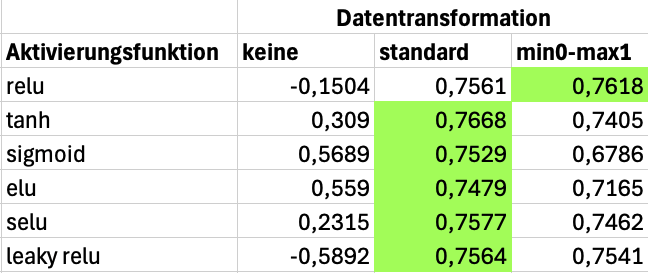
\includegraphics[width=0.4\textwidth]{Bilder/ergebnisse_aktivierungsfunktion_datentransformation.png}
    \label{tab:ergebnisse_aktivierungsfkt_transformation}
\end{table}

Wie erwartet führen die unterschiedlichen Intervalle der Featuredaten dazu, dass ein Lernen ohne Datentransformation nicht geeignet ist (siehe Tabelle \ref{tab:ergebnisse_aktivierungsfkt_transformation}). Insgesamt zeigt sich, dass die Aktivierungsfunktionen bei standardisierten Daten durch die gut konditionierten Bereiche und nur zwei hidden Layers einen geringen Einfluss auf das Lernverhalten aufweisen.

\begin{figure}
    \centering
    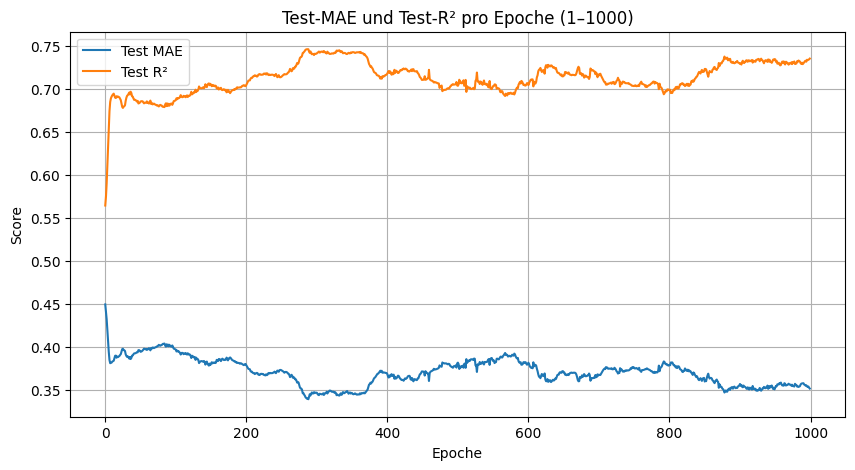
\includegraphics[width=0.6\linewidth]{Bilder/MAE_R2Test_pro_Epoche.png}
    \caption{Verlauf des MAE in \$100.000 und des $R^2$ über den Epochenverlauf}
    \label{fig:epochenverlauf}
\end{figure}

Ähnliches Verhalten kann auch bei Optimierung von Lernrate, Batch-Size und Epochenanzahl beobachtet werden. Neben einer groben Einordnung mögliche Wertebereiche:
\begin{enumerate}
    \item Lernrate: [0.001, 0.01]
    \item Batch-Size: [16, 32, 64, 128]
    \item Epochenanzahl: [200, 500]
\end{enumerate}
konnte vor allem folgendes Festgestellt werden. Die Lernrate und Batch-Size schwanken in dem oben angegeben Intervall um bis zu 3 \% im $R^2$ Testscore, was auf ein zufälliges Training hindeutet und im Folgenden durch die Varianz bei erneutem Ausführen des selben Codes zurückzuführen ist. Wie in Abbildung \ref{fig:epochenverlauf} zu erkennen ist und durch mehrere Durchläufe bestätigt wurde, sind 100 Epochen noch nicht ausreichend um ein lokales Minimum in der Fehlerlandschaft zu erkennen. Im Vergleich muss auch betrachtet, dass das Overfitting ab 500 Epochen deutlich zunimmt und dann mehr Rauschen wie Informationen gelernt werden. Auch die Anwendung einer Anpassung der Lernrate während des Trainings (LR-Schedule) führt nicht zu einem verbesserten Lernen.

\begin{figure}
    \centering
    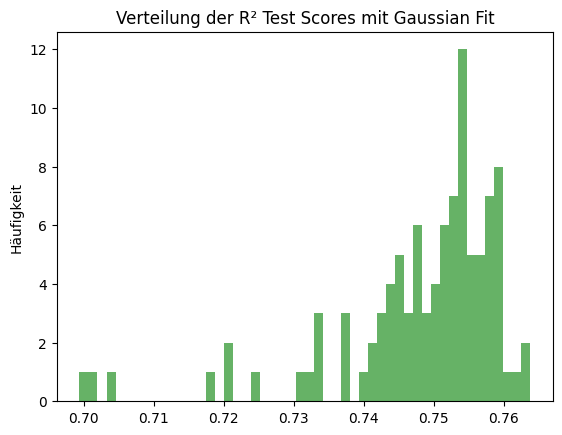
\includegraphics[width=0.4\linewidth]{Bilder/varianz_erneutes_training.png}
    \caption{Verteilung des erreichten $R^2$ Testscores über 100 Modelle}
    \label{fig:statistik_ausfuehrung}
\end{figure}

Wie bereits erwähnt ist während dem Training aufgefallen, dass ein erneutes Lernen eines Netzes zum Teil zu verschiedenen Ergebnissen führen kann. Dies ist Problematisch um eine Verbesserung mittels Hyperparameteroptimierung zu erreichen, wenn die Varianz bereits durch eine erneute Ausführung gegeben ist. Abbildung \ref{fig:statistik_ausfuehrung} zeigt die statistische Verteilung des erreichten Testscores über 100 Modelle \parencite{reproduzierbarkeit}. Daraus resultiert ein Mittelwert von 0.7481 mit einer Standardabweichung von 0.0124. Dadurch zeigt sich das vermutete Problem, dass die Hyperparameter sich nicht weiter optimieren lassen, da Sie durch die Varianz des Modells überdeckt werden. Gründe dafür sind andere Initialgewichte in Keras, unterschiedliche Ausführungsreihenfolgen auf der CPU und die Reproduzierbarkeit von Floating-Points.

\subsection{Random Search}
Da bisher nur Hyperparameter einzelnd betrachtet wurden, erfolgt ein systematischer Test mittels Random Search. Dies wird Grid Search vorgezogen aufgrund der zu erwarteten Rechenzeit und Ergebnisse der Varianten \parencite{randomsearch2012}. Über 100 Modelle zeigte sich, dass ein $R^2$ Testscore von 0.7759 erreicht werden kann. Durch eine Betrachtung der besten zehn Modellen zeigte sich, dass kein Hyperparameter verhältnismäßig oft für ein gutes Ergebnis sorgt. Dies bestätigt den hohen Zufall, der momentan im Training herrscht. Daher werden in Zukunft immer fünf Mal ein Modell mit identischen Parametern trainiert.
Ein weiteres Problem war, dass weitere Hyperparameter von Kolja parallel bearbeitet wurde, aber durch Git-Probleme ich nicht mit diesen Erkenntnissen arbeiten konnte.

\subsection{Featureselektion des Modells und Ensemble Averaging}
An dieser Stelle erfolgte eine Betrachtung der bisher erreichten Ergebnisse, um neue Ideen für weitere Verbesserungen zu erlangen. Bei der Analyse viel auf, dass hauptsächlich nur vier Features (MedInc, AveOccup, Longitude und Latitude) für den Hauspreis wichtig sind. Daher wurde ein neues Modell mit den selektierten Features trainiert. 

Es zeigt sich, dass der Score sich nicht verschlechtert, wenn das Modell nur auf vier Features trainiert wird. Somit enthalten die anderen Features keine zusätzlichen Informationen bzw. enthalten Sie genauso viel Rauschen wie Informationen. Betrachtet man das Residuen-Histogramm für vier und allen acht Features, sieht man eine gleichmäßige Verteilung um die Null herum. Ebenfalls erhalten wir eine schlankere Verteilung, welches auf eine bessere Vorhersage bzw. einen besseren Score schließen lässt (siehe Abbildung \ref{fig:featurereduzierung_histogram}).

Durch die geringeren Freiheitsgrade wird Overfitting reduziert, kein unnötiges Rauschen erlernt, und das Training vereinfacht. Die Ergebnisse lassen darauf schließen, dass die Modellleistung durch die Datenqualität anstatt durch die Modellkomplexität begrenzt ist. Das zeigt sich auch in der Abbildung \ref{fig:featurereduzierung_residuenplots}, da keine Cluster, unterschiedliche Ordnungen und kein Bias erkennbar sind \parencite{residuenanalysis2022}.

\begin{figure}[h!]
    \centering
    \begin{subfigure}[t]{0.38\textwidth}
        \centering
        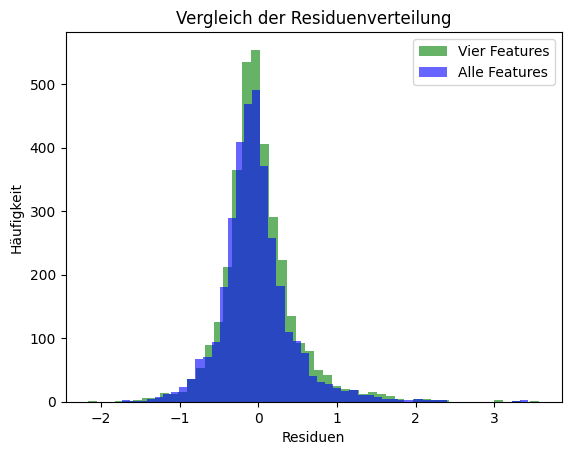
\includegraphics[width=\linewidth]{Bilder/Residuen_neu.png}
        \caption{Residuenhistogramme für acht und vier Features}
        \label{fig:featurereduzierung_histogram}
    \end{subfigure}
    \hfill
    \begin{subfigure}[t]{0.58\textwidth}
        \centering
        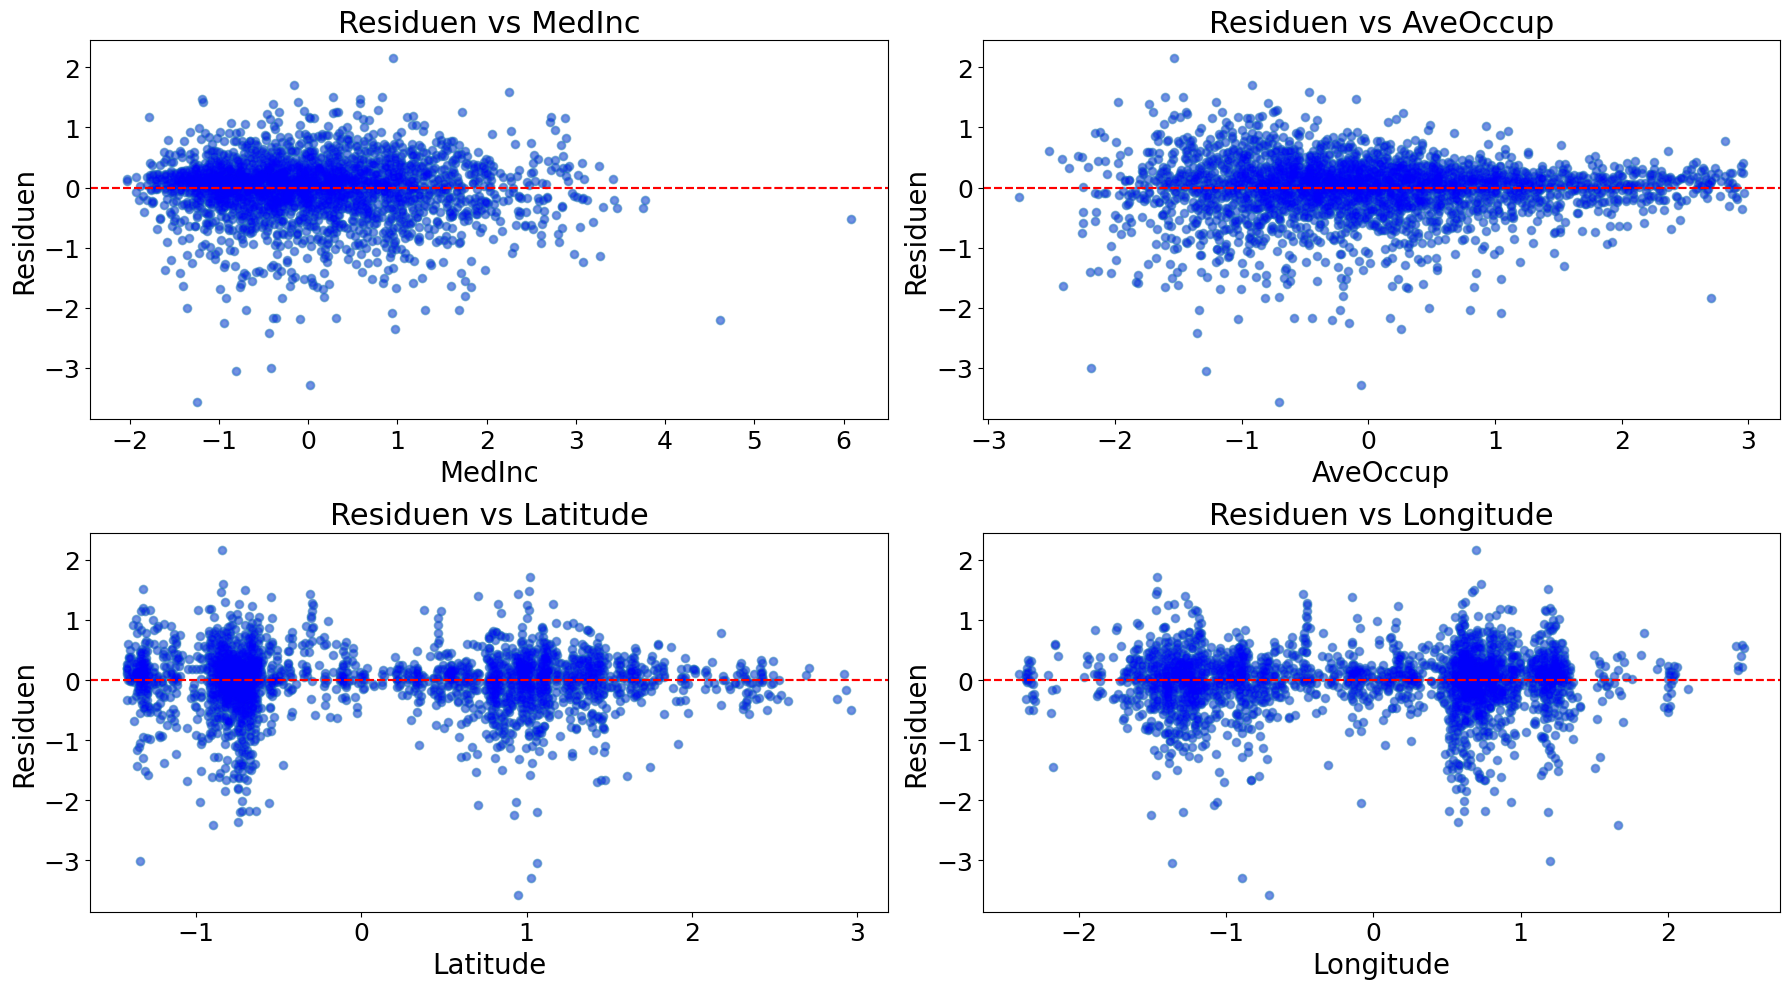
\includegraphics[width=\linewidth]{Bilder/Residuen_vier_beste_neu.png}
        \caption{Residuen für jedes der vier ausschlaggebenden Features}
        \label{fig:featurereduzierung_residuenplots}
    \end{subfigure}
    \caption{Vergleich der Residuenplots bei unterschiedlicher Featureanzahl}
    \label{fig:featurereduzierung}
\end{figure}

Mittels Ensemble Averaging \parencite{ensemblewiki2026} sollen die Vorteile der bisher betrachteten Module zusammengefasst werden. Aus einer Kombination von vier Modellen mit jeweils unterschiedlichen Hyperparamtern und Featureanzahl kann ein $R^2$ Testscore von 0.7983 erreicht werden. \parencite{ensemble_code} Dadurch zeigt sich deutlich, dass die Modelle nicht Redundant sind und exakt korrelieren.

\subsection{Zwischenstand und Ausblick}
- Random Search über alle Parameter
- Hyperparameter nicht weiter untersucht werden
- Komplexität ausreichend
- Dropout, Netzstbilisierung noch testen
- Ensemble ist gut für Verbesserung
- Ausreißer anschauen eventuell auf datenbereinigung zurückzuführen


\newpage
\section{Einschätzung der Gruppenmitglieder}

\underline{Björn Becker:}\\[1em]Positiv:\\[1em]Negativ:\\[1em]\underline{Felix Neumann:}\\[1em]Positiv:\\[1em]Negativ:\\[1em]\underline{Florian Adamczyk:}\\[1em]Positiv:\\[1em]Negativ:\\[1em]\underline{Kolja Scriba:}\\[1em]Positiv:\\[1em]Negativ:





\newpage
\section{Quellen und Hilfsmittel}
\printbibliography[heading=none]




\end{document}